\section{VL 06: Kontext Prozess II}

\subsection{Nachrichtenfluss}

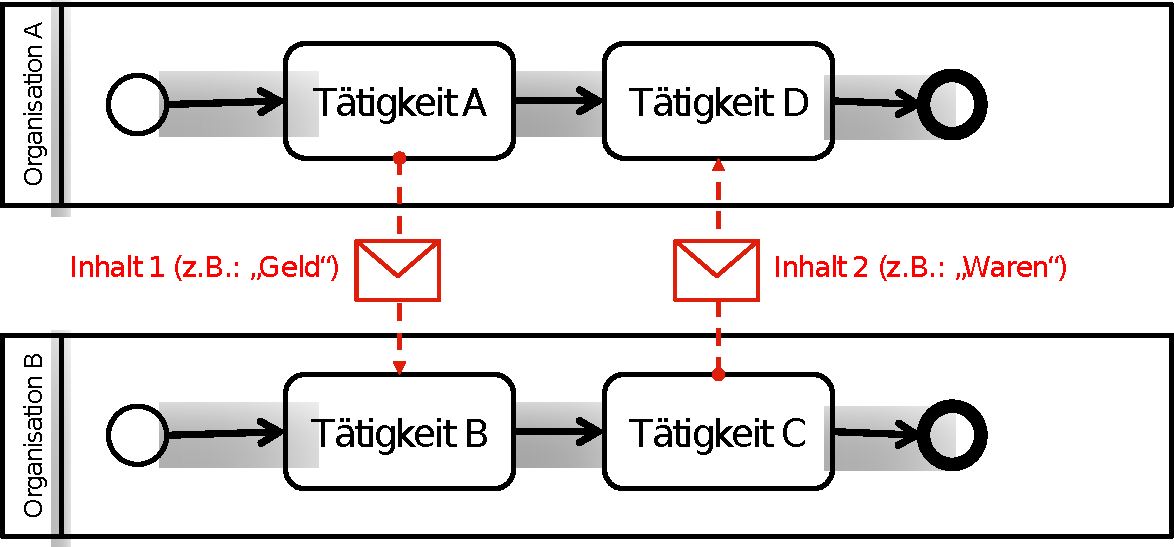
\includegraphics[width=0.7\textwidth]{6-1}

\begin{itemize}
  \item Informationsaustausch zwischen unterschiedlichen Organisationen
  \item Ein gestrichelter Pfeil A $\rightarrow$ B bedeutet dabei, dass B auf eine Nachricht von A wartet
  \item »Das Einführen von Swimlanes ist durchaus mit dem Malen von Kästchen verbunden«
\end{itemize}


\subsection{Prozessmodell am Beispiel Pizza}

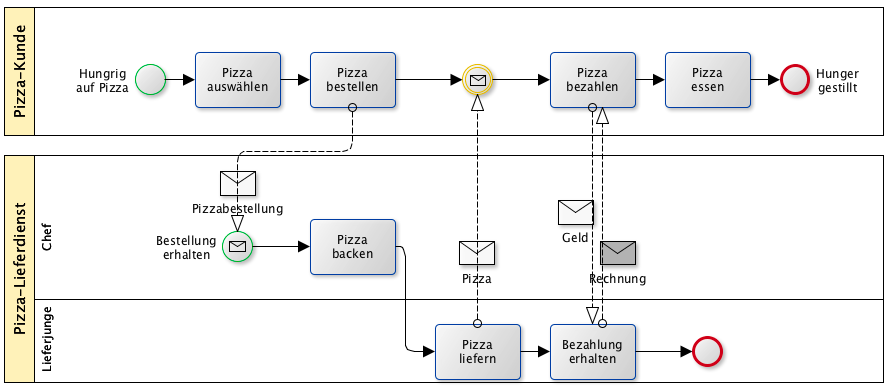
\includegraphics[width=\textwidth]{6-2}

Ein weiteres Beispiel-Modell zu Prozessmodellen (Logistik) findet sich im Foliensatz.


\subsection{Verbesserungen von Prozessmodellen}

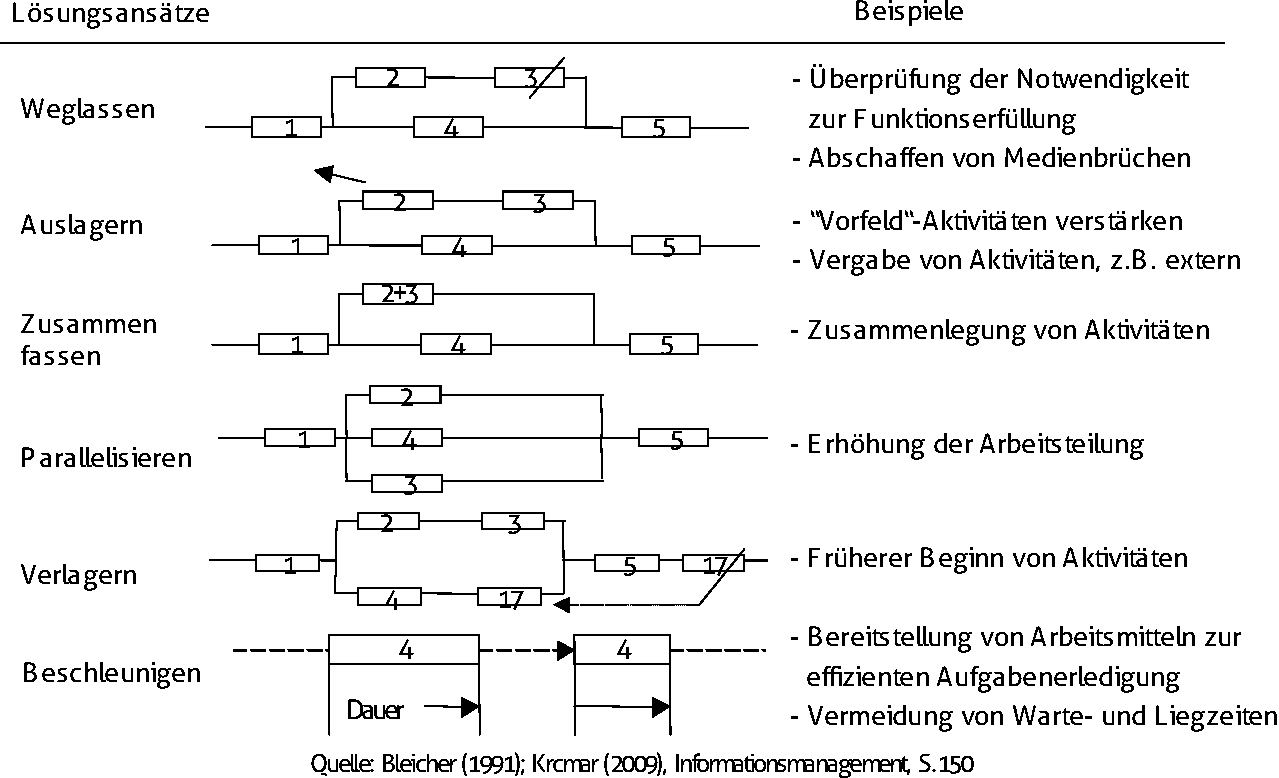
\includegraphics[width=\textwidth]{6-3}


\subsection{IT-Potenziale zur Prozessverbesserung}

\begin{tabularx}{\textwidth}{|l|X|} \hline
  IT-Potenzial     & Organisatorischer Einfluss/Nutzen \\\hline\hline
  Automatisch      & Reduktion manueller Eingriffe und Standardisierung der Prozesse \\\hline
  Informativ       & Verfügbarkeit großer Mengen detaillierter Informationen \\\hline
  Sequenziell      & »natürliche« Reihenfolge der Aktivitäten bis zur Parallelisierung \\\hline
  Zielorientiert   & Kontinuierliche Verfolgung des Prozessstatus \\\hline
  Analytisch       & komplexe Auswertung vorhandener Informationen \\\hline
  Geographisch     & Unabhängigkeit von räumlichen Gegebenheiten \\\hline
  Integrierend     & Zusammenfassung auch heterogener Aufgaben \\\hline
  Wissen schaffend & flächendeckende Verfügbarkeit von Wissen und Expertise \\\hline
  Vereinfachend    & Entfernung von Intermediären aus dem Prozess \\\hline
\end{tabularx}
